%----------------------------------------------------------------------------------------
%	PACKAGES AND OTHER DOCUMENT CONFIGURATIONS
%----------------------------------------------------------------------------------------

\documentclass[twoside]{article}

\usepackage{lipsum} % Package to generate dummy text throughout this template

\usepackage[sc]{mathpazo} % Use the Palatino font
\usepackage[T1]{fontenc} % Use 8-bit encoding that has 256 glyphs
\linespread{1.05} % Line spacing - Palatino needs more space between lines
\usepackage{microtype} % Slightly tweak font spacing for aesthetics

\usepackage[portuges]{babel}% Use portuguese symbols
\usepackage[hmarginratio=1:1,top=32mm,columnsep=20pt]{geometry} % Document margins
\usepackage{multicol} % Used for the two-column layout of the document
\usepackage{hyperref} % For hyperlinks in the PDF

\usepackage[pdftex]{graphicx}
\usepackage[hang, small,labelfont=bf,up,textfont=it,up]{caption} % Custom captions under/above floats in tables or figures
\usepackage{booktabs} % Horizontal rules in tables
\usepackage{float} % Required for tables and figures in the multi-column environment - they need to be placed in specific locations with the [H] (e.g. \begin{table}[H])

\usepackage{lettrine} % The lettrine is the first enlarged letter at the beginning of the text
\usepackage{paralist} % Used for the compactitem environment which makes bullet points with less space between them

\usepackage{abstract} % Allows abstract customization
\renewcommand{\abstractnamefont}{\normalfont\bfseries} % Set the "Abstract" text to bold
\renewcommand{\abstracttextfont}{\normalfont\small\itshape} % Set the abstract itself to small italic text

\usepackage{titlesec} % Allows customization of titles
\renewcommand\thesection{\Roman{section}}
\titleformat{\section}[block]{\large\scshape\centering}{\thesection.}{1em}{} % Change the look of the section titles

\usepackage{float}
\restylefloat{table}

\usepackage{fancyhdr} % Headers and footers
\pagestyle{fancy} % All pages have headers and footers
\fancyhead{} % Blank out the default header
\fancyfoot{} % Blank out the default footer
\fancyhead[C]{Running title $\bullet$ November 2012 $\bullet$ Vol. XXI, No. 1} % Custom header text
\fancyfoot[RO,LE]{\thepage} % Custom footer text

%----------------------------------------------------------------------------------------
%	TITLE SECTION
%----------------------------------------------------------------------------------------

\title{\vspace{-15mm}\fontsize{24pt}{10pt}\selectfont\textbf{Roofline and Matrix Multiplication PAPI Study}} % Article title

\author{
\large
\textsc{Jose Alves, Rui Brito}\\[2mm] % Your name
\normalsize Universidade of Minho \\ % Your institution
\vspace{-5mm}
}
\date{}

%----------------------------------------------------------------------------------------

\begin{document}

\maketitle % Insert title

\thispagestyle{fancy} % All pages have headers and footers

%----------------------------------------------------------------------------------------
%	ABSTRACT
%----------------------------------------------------------------------------------------

\begin{abstract}

\noindent 
This paper describes the roofline analysis of two different machines. The roofline consists in a theoretical performance model that provides visual insights on floating point computing performance. This model relates processor performance to off-chip memory traffic, giving a upper bound on performance of a kernel depending on its operational intensity. In this paper is also a study of a matrix multiplication using PAPI(Performance Application Programming Interface). With PAPI we are able to use the low-level hardware counters to identify the most accessed areas of our hierarchy of memomery as well as the operations made by our software. With the results we will present the roofline model of the machine used for the study with the conclusions obtained.

\end{abstract}

%----------------------------------------------------------------------------------------
%	ARTICLE CONTENTS
%----------------------------------------------------------------------------------------

\begin{multicols}{2} % Two-column layout throughout the main article text

\section{Introduction}

\lettrine[nindent=0em,lines=3]{T}he importance of a system's characterization is due to the need of understanding the limitations of a system, in order to make the necessary optimizations to obtain the maximum performance of a system. In order to provide a easy-to-understand performance model for floating-point programs, the Roofline was created. The Roofline indentifies an theoretical upper bound on performance on a kernel that relates if a certain opetional intensity is memory-bound, dependant on accesses of memory, or computational-bound, dependant on floating-point operational units. To comprehend the influence of different components and certain architecture characteristics a number of ceilings, both computational and memory, may be added. Since the Roofline model is better understood with a case study, a matrix multiplication problem was proposed to present the theoretical limitations of the algorithm through the model. To specify the problem in the Roofline model, a series of values were obtain from the hardware counters through PAPI(Performance Application Programming Interface). PAPI allow us to reach the low-level hardware counters and obtain information from components accessed by the program.

%------------------------------------------------

\section{Roofline}

In order to calculate the rooflines, we needed the Floating-Point(FP) Performance Peak and the Memory Bandwidth's Peak. The FP Performance Peak is obtained through the CPU information. The number of cores, their clock's frequency and the amount of SIMD(Single Instruction, Multiple Data) they can do simultaneous, provides a good approxiamation of the Performance Peak for Floating-Point operations.
To attain the FP Performance Peak we calculate the following formula:

$$\mathrm{GFlop/s_{max}} =  \#_{\mathrm{cores}} \times f_{\mathrm{clock}} \times \#_{\mathrm{SIMD}}$$\\
MacBook Pro FP Performance Peak:
$$\mathrm{GFlop/s_{max}} =  2 \times 2.8 \times 8
						 =  44.8 GFLOPS\\s$$\\
HP Pavillion FP Performance Peak:
$$\mathrm{GFlop/s_{max}} =  4 \times 1.6 \times 8
						 =  51.2 GFLOPS\\s$$\\
\\
\\
The Memory Bandwitdh Peak, being independant of the number of FP Operations per second, is a 45 degree line that demonstrates the maximum FP Operations that can be done for a given Operational Intensity. This peak is given by the memory limitations, their frequency, number of channels and bus bandwidth.
To calculate the Memory Bandwidth Peak we resolve the following formula:

$$\mathrm{BW_{max}} =  \#_{\mathrm{channels}} \times mem_{\mathrm{clock}} \times bus_{\mathrm{bandwidth}}$$\\ 
MacBook Pro Memory Bandwidth Peak:
$$\mathrm{GFlop/s_{max}} =  2 \times 1067 \times 64
						 =  17.072 GB\\byte$$\\
HP Pavillion Memory Bandwidth Peak:
$$\mathrm{GFlop/s_{max}} =  2 \times 1333 \times 64
						 =  21.328 GB\\byte$$\\

%------------------------------------------------

\section{Machines' Characteristics}

The specifications of the Machines used to sample the Roofline Model are displayed on \autoref{tab:specs}. \\The HP Pavillion dv6-2190ep was also used to run the tests the matrix multiplication test case. \\

\begin{center}
\begin{table*}[htb]
	{\small
		\begin{tabular}{|l|c|c|}
			\hline 
			 & MacBook Pro late 2008 & Pavillion dv6-2190ep \\
			\hline
			\textbf{Manufacter:} & Apple & HP \\
			\textbf{Processor} & & \\
			Manufacturer: & Intel & Intel \\
			Arch: & Core & Nehalem \\
			Model: & Core 2 Duo T9600 & i7-720QM \\
			Cores: & 2 & 4 \\
			Clock Frequency: & 2.80 GHz & 1.60 GHz \\
			FP Performance's Peak: & 44.8 GFlops/s & 51.2 GFlops/s \\
			\hline 
			\textbf{Cache} & & \\
			Level: & 1 & 1\\
			Size: & 32KB + 32KB & 32KB + 32KB \\
			Line Size: & 64 B & 64 B \\
			Associative: & 8-way & 4/8-way \\
			Memory Access Bandwidth: & 40 GB/s & 22 GB/s \\
			 & & \\
			Level: & 2 & 2 \\
			Size: & 6 MB & 256 KB \\
			Line Size: & 64 B & 64 B \\
			Associative: & 24-way & 8-way \\
			 & & \\
			Level: & - & 3 \\
			Size: & - & 6 MB \\
			Line Size: & - & 64 B \\
			Associative: & - & 12-way \\
			\hline 
			\textbf{RAM} & & \\
			Type: & SDRAM DDR3 PC3-8500 & SDRAM DDR3 PC3-10600 \\
			Frequency: & 1067 MHz & 1333 MHz \\
			Size: & 4 GB & 4 GB \\
			Num. Channels: & 2 & 2 \\
			Latency: & 13.13 ns & 13.5 ns \\
			\hline
		\end{tabular}
		}
		\caption{Machines' specifications}\label{tab:specs}
\end{table*}
\end{center}

The machines Roofline models were calculated through the values explained above. As we can see through \autoref{fig:roofline1} and \autoref{fig:roofline2} the HP Pavillion Roofline is somewhat higher than the MacBook Pro. This can be explain through the difference in the specifications between both machines.
\begin{figure*}[!htp]
	\centering
		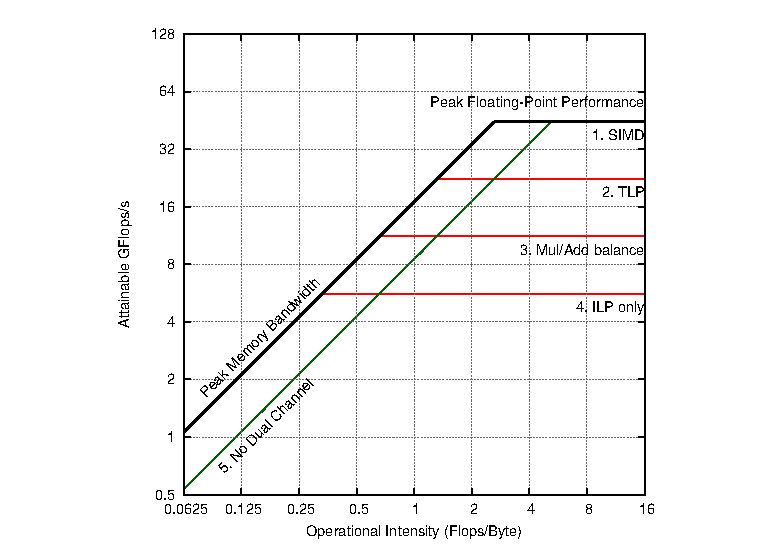
\includegraphics[width=\textwidth]{images/roofline_mbp.eps}
		\caption{Mackbook Pro late 2008 \label{fig:roofline1}}
\end{figure*}
\begin{figure*}[!htp]
	\centering
		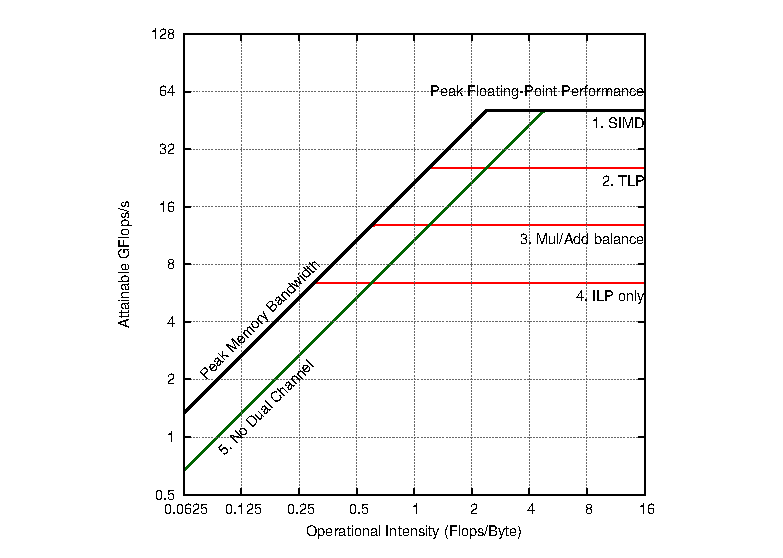
\includegraphics[width=\textwidth]{images/roofline_hp.eps}
		\caption{HP Pavillion dv6-2190ep \label{fig:roofline2}}
\end{figure*}

%------------------------------------------------

\section{PAPI Case Study}

The PAPI case study made in this project, was to analyse the performance of a \textbf{matrix multiplication} algorithm, \begin{equation}Matrix A * Matrix B = Matrix C\end{equation} wich contains a triple nested loop with the indexes i,j and k(line,column and position). Our implementation will explore the index order \textbf{i,j,k} of the triple nested loop.\\
The algorithm of matrix multiplication is presented here, in order to better understand the problem at hand.\\

\begin{verbatim}
for (i = 0; i < size; i++) {
    for (j = 0; j < size; j++) {
        for(k = 0; k < size; k++) {
            acc += matrixA[i][k] * matrixB[k][j];				
            }		
            matrixC[i][j] = acc;	
            acc = 0;
        }
    }
\end{verbatim}

As we can observe, the algorithm obtains the result of each element of matrix C through the multiplication of the line from matrix A with the corresponding column in the matrix B. As defined in the program, matrices are an array of arrays, so when is required a new element of the matrix, it fetch a line of contiguous elements from the main memory, bringing a line from the matrix. Obviously this is prejudicial to matrix B since it needs the elements of a column and not from a line, to fix this problem we expirement running the test for both the naive implementation, and one that calculates the transpose matix B and runs the algorithm throught it.  \\
To note that he implementation produced to calculate the matrix multiplication was made in C and compiled with Optimization level 1 (-o).

\subsection{PAPI Specifications}
To measure the implementation's perfomance, hardware counters were used. To gather the information of these counters, as stated above, PAPI was used. Although able to obtain the low-level hardware counters results, is still needed to  identify wich to gather as well as make sure they are available in the system. To obtain the needed information, the following counters were used:
\begin{description}
\item[PAPI \_TOT\_CYC] Total number of cycles;
\item[PAPI \_TOT\_INS] Instructions completed;
\item[PAPI \_LD\_INS] number of load instructions;
\item[PAPI \_SR\_INS] number of store instructions;
\item[PAPI \_FP\_OPS] Floating point operations;
\item[PAPI \_FP\_INS] Floating point instructions;
\item[PAPI \_L1\_DCA] L1 data cache accesses;
\item[PAPI \_L1\_DCM] L1 data cache misses;
\item[PAPI \_L2\_DCA] L2 data cache accesses;
\item[PAPI \_L2\_DCM] L2 data cache misses;
\item[PAPI \_L3\_DCA] L3 data cache accesses;
\end{description}

Four tests, as we can see in \autoref{tab:testcases}, were chosen to run in the two different version(naive and transpose). Each test was run four times, with the best execution time being select as long as the range was no larger than five per cent from the other three. To measure the influency of accessing each layer of the memory hierarchy each test fits in a different level(L1, L2, L3 and RAM).   
\\
\begin{table*}[!htp]
	\center{
	\begin{tabular}{|l|l|l|}
		\hline
		\textbf{Memory Level} & \textbf{Size of } \\
		\hline
		L1 & 32 KB \\
		L2 & 256 KB \\
		L3 & 6 MB \\
		RAM & 7.68 MB \\
		\hline
	\end{tabular}
	\caption{Test cases}
	\label{tab:testcases}
	}
\end{table*}

%------------------------------------------------

\section{Results}

To measure the data cache misses the counters PAPI\_L1\_DCM and PAPI\_L2\_DCM were used.

\begin{figure*}[!htp]
	\centering
	\begin{minipage}[t]{0.5\linewidth}
		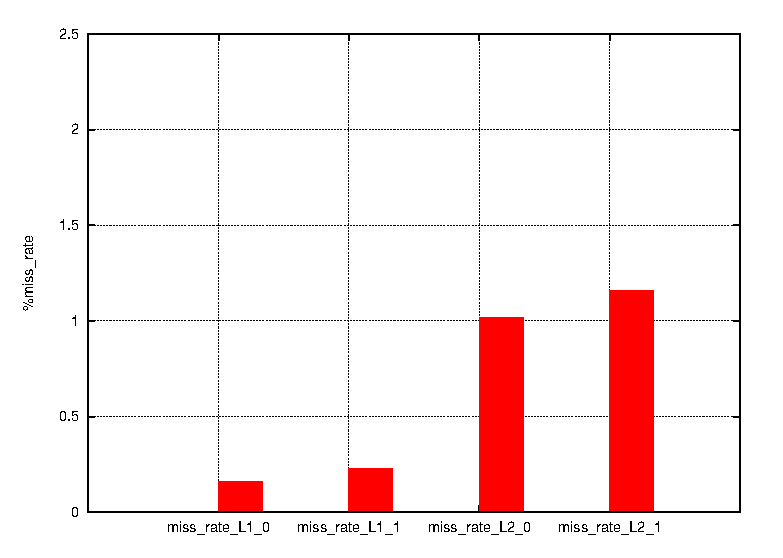
\includegraphics[width=\textwidth]{images/caches.eps}
		\caption{Percentage of Cache Misses \label{fig:cache1}}
	\end{minipage}
\end{figure*}

The \href{fig:cache1} graphic shows an increase of percentage of misses with the optimized version, they are misleading. The \href{fig:cache2} graph shows that although the percentage of misses increased, the total of misses didn't because the number of accesses also droped.

\begin{figure*}[!htp]
	\centering
	\begin{minipage}[t]{0.5\linewidth}
		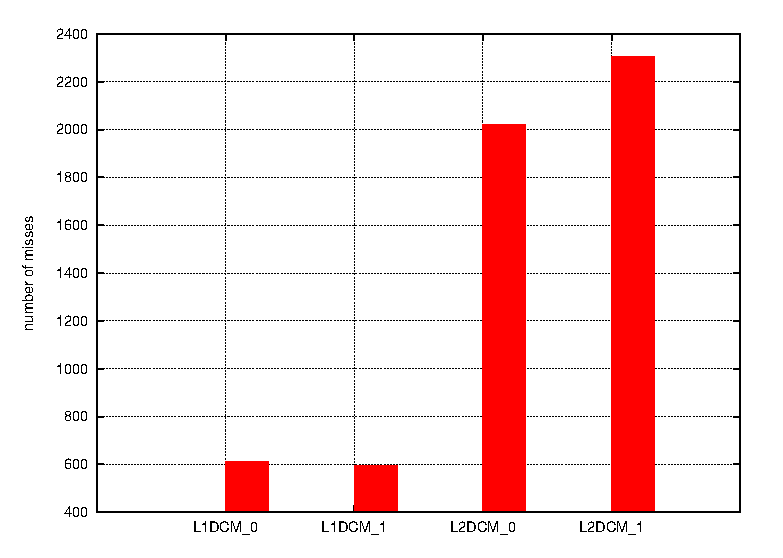
\includegraphics[width=\textwidth]{images/misses.eps}
		\caption{Number of Cache Misses \label{fig:cache2}}
	\end{minipage}
\end{figure*} 

Usage of both levels of cache was estimated with specific counters. PAPI\_L1\_DCA and PAPI\_L2\_DCA provided the number of data accesses to the caches.

Before the results were out, it was expected a decrease of cache accesses from version one to version two of the algorithm.

\begin{figure*}[!htp]
	\centering
	\begin{minipage}[t]{0.5\linewidth}
		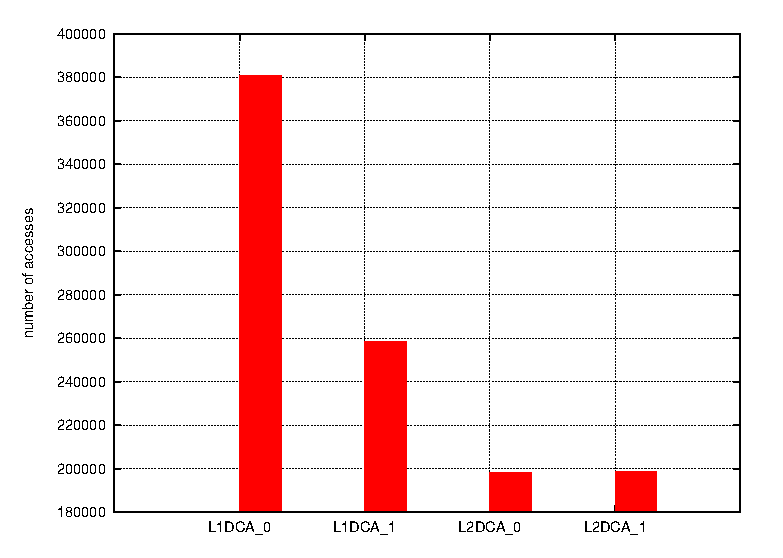
\includegraphics[width=\textwidth]{images/totals.eps}
		\caption{Number of Memory Accesses \label{fig:cache3}}
	\end{minipage}
\end{figure*}

As we can see in \href{fig:cache3} graph, the number of access to cache drops significantly from the first version to the second version while running with the L1 Cache Test. Though in the second test, the L2 Cache, the number of accesses slightly increased.



%----------------------------------------------------------------------------------------
%	REFERENCE LIST
%----------------------------------------------------------------------------------------

\begin{thebibliography}{99} % Bibliography - this is intentionally simple in this template

\bibitem{roofline}
	\texttt{\small
	Roofline: An insightful Visual Performance Model for Floating-Point Programs and Multicore Architectures}	\\
	\emph{Samuel Webb Williams, Andre Waterman, David A. Patterson}	\\
	23th November 2012

\bibitem{ark}
	\texttt{\small
	http://ark.intel.com/products/ 35563/Intel-Core2-Duo-Processor- T9600-6M-Cache-2\_80-GHz-1066-MHz-FSB}	\\
	\emph{Intel{\textregistered} Core {\texttrademark} 2 Duo Processor T9600 (6M Cache, 2.80 GHz, 1066 MHz FSB)}	\\
	{\copyright}Intel Corporation	\\
	23th November 2012

\bibitem{ark2}
	\texttt{\small
	http://ark.intel.com/products/43122/ Intel-Core-i7-720QM-Processor- 6M-Cache-1\_60-GHz}	\\
	\emph{Intel{\textregistered} Core {\texttrademark} i7-720QM Processor(6M Cache, 1.60 GHz)}	\\
	{\copyright}Intel Corporation	\\
	23th November 2012

\bibitem{crucial}
	\texttt{\small
	http://www.crucial.com/store/ ListParts.aspx?model=MacBook\%20Pro \%20\%28Early\%202008\%20and \%20Late\%202008\%29}	\\
	\emph{Computer memory upgrades for Apple MacBook Pro (Early 2008 and Late 2008) Laptop/Notebook from Crucial.com }	\\
	{\copyright} Micron Technology	\\
	24th November 2012

\bibitem{crucial2}
	\texttt{\small
	http://www.crucial.com/store/ listparts.aspx?model=Pavilion \%20dv6-2190ep\&Cat=RAM}	\\
	\emph{Computer memory upgrades for HP - Compaq Pavilion dv6-2190ep Laptop/Notebook from Crucial.com}	\\
	{\copyright} Micron Technology	\\
	24th November 2012	 
\end{thebibliography}

%----------------------------------------------------------------------------------------

\end{multicols}

\end{document}
